% !TeX root = ../thuthesis-example.tex

\chapter{国内外研究现状}
传输速率控制策略作为网络应用领域重要的决策任务,已经在多年的研究下累积了许多重要工作。本章节将根据研究挑战,将相关工作分类为针对应用场景需求异质性的研究和针对策略环境性能适配差异性的策略研究两个方面分别介绍传输速率控制策略的研究发展,为传输速率控制策略的问题分析和方法研究提供基础。此外,本章还简要介绍了有关强化学习背景的相关工作。

\section{针对应用场景需求异质性的研究}
应用场景需求异质性是指由于媒体系统的服务目标和对象不同所带来的差异。通过利用这种异质性,可以有效地提升服务目标的用户体验质量。目前有很多工作针对定义用户体验质量展开研究;部分工作尝试揭露某特定应用下的独有差异性,为算法优化提供了有效的重要参考指标。

\subsection{用户体验质量的研究与定义}
用户体验质量(Quality of Experience,QoE)的研究是实时通信系统中用于评估服务质量的重要一环。它为如何设计系统、如何分析系统性能和如何评价系统实现效果带来指导性作用。根据林闯\cite{林闯2012用户体验质量}等人的研究,用户体验质量可以被定义为在用户角度对于整个服务质量的评价,包括了主观因素和客观服务质量指标(Quality of Service,QoS);QoE的影响因素也可根据该研究分为环境、用户和服务三类,如图\ref{fig:Qoedef}所示。

\begin{figure} [ht]
\centering
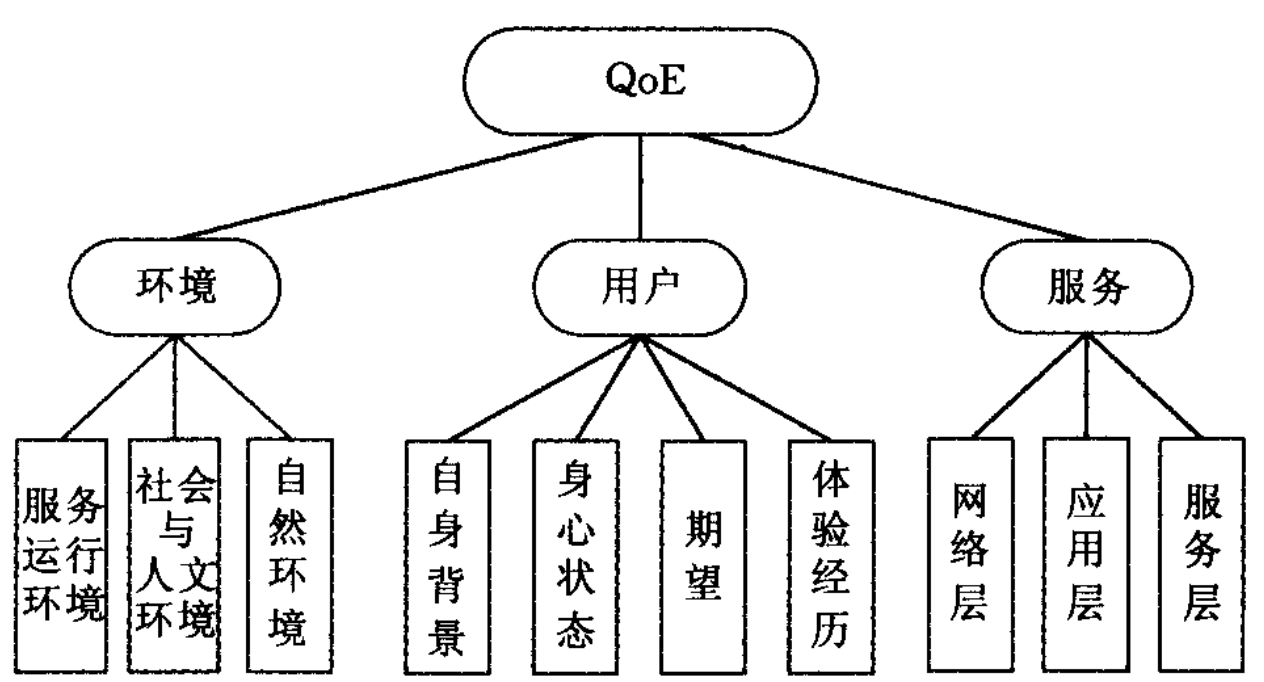
\includegraphics[width=0.7\textwidth]{figures/chap02/QoE.png} 
\caption{QoE中包含的可考虑因素列举\cite{林闯2012用户体验质量}}
\label{fig:Qoedef}
\end{figure}

新的应用类型因为提供服务需求的改变,用户主观的感知质量会因此而产生影响。同时,用户体验质量能够作为最终优化目标,指导系统优化工作。当前已经有多种类型的,从不同的场景与角度出发的QoE评判方式。例如,内容服务提供商可能将使用时长作为关键的QoE指标\cite{CTR洞察},因为高用户留存率可以带来高经济收益;而对于个人用户,当遇到系统抖动时,呈现内容品质降级的过渡策略(例如画面跳过、画面预测、自适应比特率或重新加载)可能会对于用户感受质量造成非常大的影响。

一部分工作会试图在模拟网络拓补下的开展用户主观评分,获取直接的用户真实反馈。这类工作在局域网的拓扑上利用网络模拟器(如NetEm\cite{hemminger2005network}, Mahimahi\cite{netravali2015mahimahi}, ns-3\cite{henderson2008network}或其他工具)模拟真实的网络可能遇到的环境,并通过用户五分制打分(MOS)\cite{林闯2012用户体验质量}的方式衡量某些因素对用户体验质量的影响。目前已有在云游戏、视频业务和其他类型的实时服务商开展此类研究的工作\cite{jarschel2011evaluation,ahmad2023significance,zadtootaghaj2018modeling,zhang2019e2e,lindstrom2020cloud}。工作引入了多种因素的端到端网络,例如高延迟、抖动、丢包、带宽控制和资源分配,以及视频特性中的码率等因素,衡量每个因素的影响多少。参与者会被要求在一个阶段后对前述感受进行五分制的打分。

另一种方式是识别重要指标并建立一个质量预测模型给出打分。这类工作通过大规模的数据测量,尝试识别新的应用中特有的能够反映用户QoE的指标,并根据这些指标建立预测模型。这一类工作包括\cite{balachandran2013developing,cheng2023rebuffering,zhu2022eyeqoe},分别应用于视频观看、短视频点播和VR全景视频。用于评估QoE的指标在建立预测模型时可能会有多个,包括实时通信系统中的诸如时延、抖动通用的指标,到用户退出率、眼动位置坐标等应用特有数据,这些数据共同作为模型的输入,构成最后的QoE预测模型。

还有一部分工作着重研究了画质和码率切换对于用户体验带来的负面影响的具体衡量方法。\cite{slivar2016cloud,jamshidi2022deep,utke2022ndnetgaming}中通过将画面灰度的峰值信噪比(Peak Signal-to-noise ratio,PSNR)或视频多方法评估融合(Video Multimethod Assessment Fusion, VMAF)指标值区间映射入各自的长短时记忆模型(Long Short-Term Memory,LSTM),获得以秒为粒度的预测用户质量数据。
\cite{mao2017neural,huang2019comyco,nathan2019end}在对于各自的模型进行评估时使用式\eqref{equation-qoe}进行QoE中品质降级的过渡策略(画面跳过、画面预测、自适应比特率或重新加载)带来的影响的量化衡量:
\begin{equation}
    QoE = \sum_{n=1}^{N}q(R_n) - \mu \sum_{n=1}^{N}q(T_n) - \sum_{n=1}^{N-1}\lvert q(R_{n+1})-q(R_n) \rvert,
\label{equation-qoe}
\end{equation}

其中, $N$ 代表视频块的数量,$R_n$ 代表第 $n$ 个视频块的比特率,$T_n$ 代表第 $n$ 个视频块重加载的时间,最后一项代表比特率切换的影响,亦被称作为流畅度。 $\mu$ 则是经验值罚项。


\subsection{特定应用需求差异性分析工作}
E2E\cite{zhang2019e2e}对互联网上流量吞吐提出了大型范式,涵盖了所有涉及用户参与的连接请求,其核心思想在在于挖掘用户对于应用需求的QoE异质性。对于云游戏、视频会议、360$^{\circ}$视频等不同种类的应用,现有的工作对它们展开了针对性的探索。ClayPool等人尝试描述网络游戏中玩家对于其操作响应和画面变化延迟的敏感性\cite{claypool2006latency,claypool2010latency},使用网络时延对于用户表现分数的影响说明了游戏内容对时延要求差异的存在和定性,并给出了要求的极端下限阈值。EyeQoE\cite{zhu2022eyeqoe}在VR设备的使用过程中和360$^{\circ}$视频的播放对用户的眼球运动进行追踪,对具体的眼球运动分类并捕捉运动模式,以预测其运动轨迹和感知质量。Michael等人尝试开展对于用户的主观测试\cite{jarschel2011evaluation},并发掘了游戏节奏是有差异性的,这种差异性造成了对网络时延控制、丢包控制等优先性的偏好不同。Cheng等人在大型短视频服务提供商的数据集上进行了广泛的用户行为研究\cite{cheng2023rebuffering}。测量数据表明,不同的视频流内容虽然在遇到卡顿时会让用户不满,进而增加用户的提前退出率,但是它们的概率是有所不同的,体现出不同视频流卡顿对QoE影响的差异性。


\section{环境性能适配差异性的策略研究}
环境性能适配差异性是指由于所处网络的环境所固有的属性有所不同带来的差异。这种差异性通常是由于物理层的链路特性、网络使用所处的环境、网络应用的差异,或与不同时段带宽链路的利用率等有直接相关性。针对这样的差异性进行研究,可以针对于网络的特性更好地做出相适配的决策,进而提供更可靠的网络传输保障和更好的服务质量。目前有大量工作针对于此差异性展开了深入和广泛的研究。

\subsection{适用于差异化环境性能的速率控制算法研究}
速率控制是一个重要的传输速率控制策略,工作于网络的传输层,在实践应用时有时会交由应用层完成其功能。它的目的是为了保证传输的可靠性和效率。一个常见的网络点对点连接可以抽象为一个如图\ref{fig:sending} \cite{author2024performance}所示的结构:发送器和接收器对应两条不同的路由,而在链路上会遇到瓶颈带宽。发送器需要控制发送的速率以确保一定的带宽利用率才能保证传输效率,并避免其过大造成的发送失败。“速率控制”通常被理解为可靠传输控制协议(即TCP协议)中发送端根据网络状况和接收窗口的情况实行发送包的控制,或是应用层根据接收缓冲区的状况进行的码率发送选择。在TCP拥塞协议的约定下,接收方必须对于每个接收到的包回应一个ACK信号(部分情况下,多个包可以使用ACK聚合回应一次),发送方也需要等待发送的前序包确认收到后再发送后续包。但在实时通信系统中,使用可靠传输协议的等待ACK信号会大幅降低系统的实时性,因此多数系统和应用在传输层使用了数据报的方式进行传输,而将可靠传输的任务交由应用层完成,例如QUIC\cite{langley2017quic}协议。在这种情况下,协议根据流式媒体内容的特性针对性进行拥塞控制。同时由于通信系统中网络时延和网络抖动带来的负面影响占据了总时延比重的主要部分\cite{yuan2022understanding},大量发送速率控制和流量管控工作集中于这一环节,针对于不同的环境性能进行改善。系统整体的性能亦随速率控制算法的进步而得到改善。

\begin{figure} [ht]
\centering
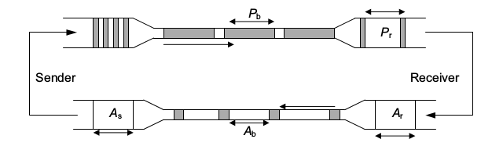
\includegraphics[width=0.8\textwidth]{figures/chap02/sending.png} 
\caption{速率控制的工作环境和其目的\cite{author2024performance}}
\label{fig:sending}
\end{figure}


速率控制通常可以根据其探测所依赖的关键信息进行区分,例如基于网络丢包(loss-based)信号、基于时间延迟大小(delay-based)信号、或是基于时延-带宽积(Bandwidth-Delay Product)信号等。除外,速率控制还可依照建立的不同的理论进行区分,例如延迟排队理论建模、固定规则、启发式算法、预训练监督学习模型方法、强化学习和基于用户感知的方法等。本章节将结合多个方面,对现有的速率控制算法展开。本章节还将会从拥塞控制的特性和适配环境角度切入进行总结。

基于网络丢包(loss-based)的拥塞控制主要探测超时未收到确认信号的包数量。根据某一时间段内的丢包率推断出网络遇到了多大程度的拥塞,并及时采取措施缓解拥塞。Tahoe\cite{jasim2018old}, Reno\cite{yang2000general}和New Reno\cite{fall1996simulation}是经典的基于网络丢包的速率控制算法,它们都使用了慢启动(从低阈值开始指数增长拥塞窗口)、拥塞避免(临近预测的拥塞阈值时,线性增长拥塞窗口)、快重传(丢包后乘法降低至低值后再上升)的方式进行拥塞控制。它们三者的区别是Reno相比于Tahoe多出了快恢复算法,避免在丢包后回到慢启动阶段,降低传输效率;New Reno则改进了快恢复机制,避免单次拥塞的发生被认为是多次。根据其拥塞方法的控制原理,它们适用于相对时延不那么敏感的任务和网络缓冲区较大的任务,以及要求获得更高的吞吐量的任务。

BIC-TCP\cite{xu2004binary}和Cubic\cite{ha2008cubic}是另外两个相似的基于网络丢包的速率控制,使用窗口增长函数完成窗口的估测,Cubic使用一个奇数阶多项式修正窗口增长函数,增加了窗口增长的稳定性,避免过激带来丢包。Cubic也是目前Linux内核中默认采用的拥塞控制算法。相比于Reno,Cubic类的算法能够更快地恢复拥塞窗口。上述的Reno、Cubic都是基于一个固定规则的方法,具有极佳的稳定性。

基于测量时延(delay-based)的拥塞控制主要基于探测包发送到到达的时间或其计算后的元素。通常来说,从发送端向接收端的发送路径和从接收端向发送端的发送路径应被视作两条异质化的、无相关性的链路,这是因为它们经过的路由可能不同,或即使相同网络状况也有所差异,网络带宽有所不同。但是,由于测量手法限制,实际测量时会根据往返时延(Round-Trip Time,RTT)的一半作为时延的估测使用,判断网络的状况。还有部分算法会使用往返时延对单位时间$T$的微分($\frac{dRTT}{dT}$),即包到达时间间隔的差异作为衡量标准。TCP Vegas\cite{brakmo1994tcp}使用连接中数据包的RTT决定发送速率和探测带宽。Google于2015年提出的BBR\cite{cardwell2016bbr}亦使用了这样的思想。作者认为,由于缓存技术的发展,网络这一本该即用即走的链路因为路由设备和中继设备的缓存装置使之有了存储的功能。由于网络设备处理能力有限,在应用发送包不断增加时,首先到达处理能力瓶颈。此时发送出的包容量为一个时延带宽积(BDP)。此时如果发送速率继续上升,会在网络存在的缓冲区中存储。此时会导致发送包处理的队列,造成ACK回复的时间变长,此时体现为测量到的往返时延(RTT)增加;直至网络缓冲区也被填满,此时就会产生丢包。BBR使用固定的时段探测带宽,并根据结果对于发送速率进行乘以固定因子的挑战,不断自适应网络状况。这一类方法也使用了一些固定的规则,带来可靠的同时适用于需要较低时延,但不存在较多竞争的任务。

而Copa\cite{arun2018copa}是一种默认工作在以传输时延作为探测信号的发送速率控制方法,保证低时延应用的传输;然而,在探测到其他丢包流竞争的时候,Copa会切换到以丢包为探测信号的工作模式中,以便在多流竞争中取得相对的公平性。这是由于当基于丢包控制算法与基于时延为信号的控制算法在一个瓶颈带宽时,时延瓶颈通常会先于丢包发生,造成算法竞争的不公平。Venkat Arun等人在工作\cite{arun2022starvation}中揭露了当前所有基于测量时延的拥塞控制算法中存在的多流竞争导致的部分算法的饥饿的现象,通过一个网络模型复现了多个前述算法在竞争中存在的缺陷,并给出了饥饿产生和拥塞算法收敛的推导,揭示了问题的本质。Copa对于网络的拥塞控制服务基于的原理是排队论中的 M/M/1 模型,建立在将包到达时间视为泊松过程(Poisson process)这一假设上对于发送速率进行优化,进而使网络利用率最高。这种算法能够兼顾低时延与公平性,适用于多流竞争情况下的低时延保障场景与任务。类似地,WebRTC中采用的GCC\cite{carlucci2016analysis}使用了混合丢包与时延策略的算法同时借助两种信息进行判断。延迟间隔经过多个滤波器后得到一个发送速率,同时丢包探测器同步进行丢包检测,同样给出一个发送速率,选择两者较小者实行。

SQP\cite{ray2022sqp}使用了贴近于视频帧的发送策略,即以帧为单位,单次发送时将一帧的多个包在短时间内发出,并根据收到的ACK时间戳估测带宽的使用情况,恰好用作带宽探测。SQP根据每帧的第一个包的发送时刻与上一帧最后一个包的接收时刻之间的差值作出带宽过度/不足利用的估计,并根据该时间间隔完成发送速率的调整。这种方法适用于低时延视频传输的环境。

PCC-Allegro\cite{dong2015pcc}和PCC-Vivace\cite{dong2018pcc}将时间切分为检测间隔(Monitor Intervals),使用一个效用函数完成拥塞控制,内包含对于时间间隔与丢包情况的权重估计。而它们的区别在于PCC-Allegro会使用探测性决策方法决策发送速率,是基于传统方法的策略;而PCC-Vivace则使用了在线学习,通过梯度在线优化算法完成发送速率的调整。PCC-Expr则是另外一个PCC系列的变种,旨在提高通过率和延迟控制之间的平衡,特别是在需要极低延迟的环境中。

得益于强化学习在决策类任务的优异性能表现\cite{mnih2013playing},使用强化学习的速率控制方法也在近年来出现和发展。Orca\cite{abbasloo2020classic}便是一个基于强化学习的拥塞控制方法,他指出了当前纯学习型拥塞控制设计的不足,并表明选择深度强化学习能够从原始数据中提取出高度有效的信息,并与环境互动,逐步做出决策。Orca通过将含有吞吐量、时延和带宽利用情况的指标量化为一个奖励值作为强化学习的学习目标,并使用了精细设计的模块,成功将强化学习应用于拥塞控制任务中,在全球范围的测试平台上部署的Orca实现了良好的效果。Aurora\cite{jay2019deep}使用了类似的强化学习方式实现了拥塞控制,并尽可能保障了多流竞争之间的公平性与安全性。这类方法使用网络变化大、连接时间长,需要时间适应的独特特性网络,但对于部署算法的要求较高。 R3Net\cite{fang2019reinforcement}使用了相同的方法但设计了差异化的模型以便更好地提取出网络信息,服务于实时通信系统中的发送速率控制或是传输层的拥塞控制。

随着强化学习的发展,强化学习被用于速率控制的情况越来越多,尤其是RTC系统中的实时速率控制。为此,微软推出了一个仿真平台OpenNetlab\cite{eo2022opennetlab},它将一个RTC仿真模拟器封装,并抽离出对接强化学习算法的接口,还提供真实部署在各地的服务器用于测试性能。ReCoCo\cite{markudova2023recoco} 是使用该仿真平台构建的,专用于超低时延的实时通信任务的基于强化学习的发送速率控制模型。


亦有一部分工作基于场景总结后的用户感知特性完成算法控制的优化。例如,PACC\cite{peng2023pacc}是使用了卷积神经网络(Convolutional Nerual Network,CNN)构建画面的传感器模块,从而有选择地高质量传输更重要的部分。这样的策略与上节的QoE形成更紧密的耦合。


除此以外,环境性能适配差异性还体现在更细粒度的具体场景上。比如,在高速铁路上,由于快速的移动,基站部署的稀缺,会导致收发消息的链路可靠性衰减。针对于这样与常规环境不同的差异性,POLYCORN\cite{ni2023polycorn}和Cellfusion\cite{ni2023cellfusion}使用了多径改善了户外或高速铁路上移动时的信道质量。通过不同运营商提供的两个链路和自适应的补偿机制完成了发送。这一类针对不同应用而采用多链路方式弥补的工作也有很多,比如针对于视频会议的Converge\cite{dhawaskar2023converge}和Twinstar\cite{wang2023twinstar}。

\subsection{适用于不同场景的自适应码率算法研究}
自适应码率也是发送速率控制算法中的重要一部分。相较于工作在传输层的拥塞控制类型的发送速率控制任务,它有的独特特点是更粗粒度的决策和有限的决策选择。自适应码率流式传输算法的工作原理如图\ref{fig:abrteaser}所示。

\begin{figure} [ht]
\centering
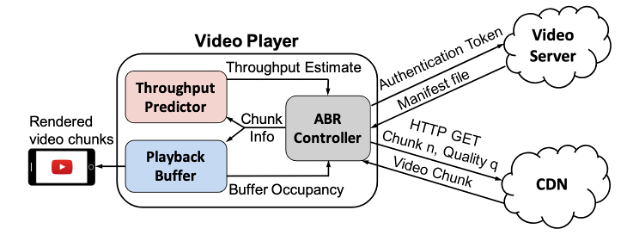
\includegraphics[width=0.75\textwidth]{figures/chap02/abrteaser.png} 
\caption{自适应码率流式传输系统的工作原理\cite{mao2017neural}}
\label{fig:abrteaser}
\end{figure}


自适应码率流式传输系统根据网络的实时带宽情况动态选择合适的码率来传输视频内容。每个视频被预先转码为多个不同码率的片段(chunk),每个片段代表视频中的一个时间段,大约几秒。在播放过程中,系统根据当前网络状况和客户端的缓存状态,选择一个合适的码率进行下载。当网络带宽较好时,系统会选择较高的码率以提供更高质量的视频体验;而在网络带宽受限时,系统则会选择较低的码率以避免视频卡顿和缓冲现象。自适应码率算法通过定期监测网络带宽和视频播放状态,调整发送码率以确保视频流畅播放。自适应码率流式传输算法通常基于反馈控制机制,如图\ref{fig:abrteaser}中的控制器所示(ABR Controller)。客户端通过定期发送网络带宽反馈给服务器,服务器根据这些反馈信息决定下一个时间段内应选择的码率。常见的自适应码率算法包括基于带宽估计的算法、基于延迟的算法以及混合算法等。每种算法都有其优缺点,需要根据具体应用场景进行差异性的选择。

经典的自适应码率流式传输算法有模型预测控制方法(Model Predictive Control,MPC)\cite{yin2015control}方法,一种传统的基于规则的方法。这种方法利用动态规划的方式,将吞吐量估计和关于缓冲区占用的观测信息用于选择在未来一段时间内最大化给定 QoE(用户体验质量)指标的码率。除外,基于缓冲区的自适应码率算法(Buffer-Based Algorithm,BBA)\cite{huang2014buffer}基于客户端的缓冲区占用情况来调整视频的码率,而不是依赖于复杂的容量估计。通过这种方法,能够在不依赖复杂的容量预测的情况下,减少 10\% 到 20\% 的重缓冲率(rebuffer rate)。BOLA(Buffer Occupancy based Lyapunov Algorithm)\cite{spiteri2020bola}是一种基于缓存占用率的自适应码率算法,能够通过控制缓存的上下限来避免缓冲过多或过少,从而确保视频的流畅播放。以上三种方法都是较为传统的,基于固定规则的算法,具有较好的稳定性,但可能缺乏灵活性。

Pensieve\cite{mao2017neural}是使用强化学习完成自适应码率任务的代表。该算法使用了一个可并行的演员-评论家(Actor-Critic,加并行后表示为A3C)进行码率选择的决策。它能够自适应调整策略,学习不同网络条件下的最佳行为,从而实现流媒体传输的最优体验。Genet\cite{xia2022genet}是在Pensive基础上进一步改良的自适应码率任务,并扩展到了更多发送速率控制相关的人物上。它的改良主要是利用了课程学习的方式,让强化学习的过程从较简单的内容逐渐转向复杂的内容。



\subsection{差异性对比与工作范式研究}
在速率控制算法的发展基础上,一个庞大的历史可用库得以累积。为了统计、分析这些速率控制方法的性能以及站在更大的角度审视它们,性能对比的工作和范式规划的工作被提出。

近年来预训练大模型的出现为这一类任务提供了新的思路。得益于大模型强大的推理和决策能力,NetLLM\cite{wu2024netllm}提出了“一个模型适用所有网络任务”,亦包括了自适应码率的任务。为了适配码率的时序数据,NetLLM使用了一个多模态编码器,将网络状态时序信息编码进大模型的嵌入层;经过大模型的前向传播后限定输出头以准确地选择最终的码率。由于大模型丰富的经验和知识,NetLLM在实验中取得了优异的表现,为速率控制任务提供了崭新的思路。同样使用预训练大模型的还有LLM-ABR\cite{he2024llm},但采取了不同的思路。LLM-ABR选择让大模型生成出可用的ABR策略,并通过一系列检测和性能测试后使用,进而构建了一个策略创建范式。Nada\cite{he2024designing} 在LLM-ABR基础上进一步改进,扩展到更多网络任务上。


除此以外,许多性能对比的工作为海量的拥塞控制、自适应码率算法提供了真实的部署环境和分布在全球各地的测试平台。Pantheon\cite{yan2018pantheon}和ccBench\cite{abbasloo2023internet}是对于已有算法的部署和测试,提供了一个强大的、真实的、全面的测试平台。Puffer\cite{yan2020learning}则是ABR算法的性能测试平台。部分拥塞控制算法的性能测试的结果和自适应码率的性能测试结果如图\ref{fig-mea-ccabr}所示。

\begin{figure}[ht]
\centering
\begin{subfigure}[t]{0.49\linewidth}
  \centering
  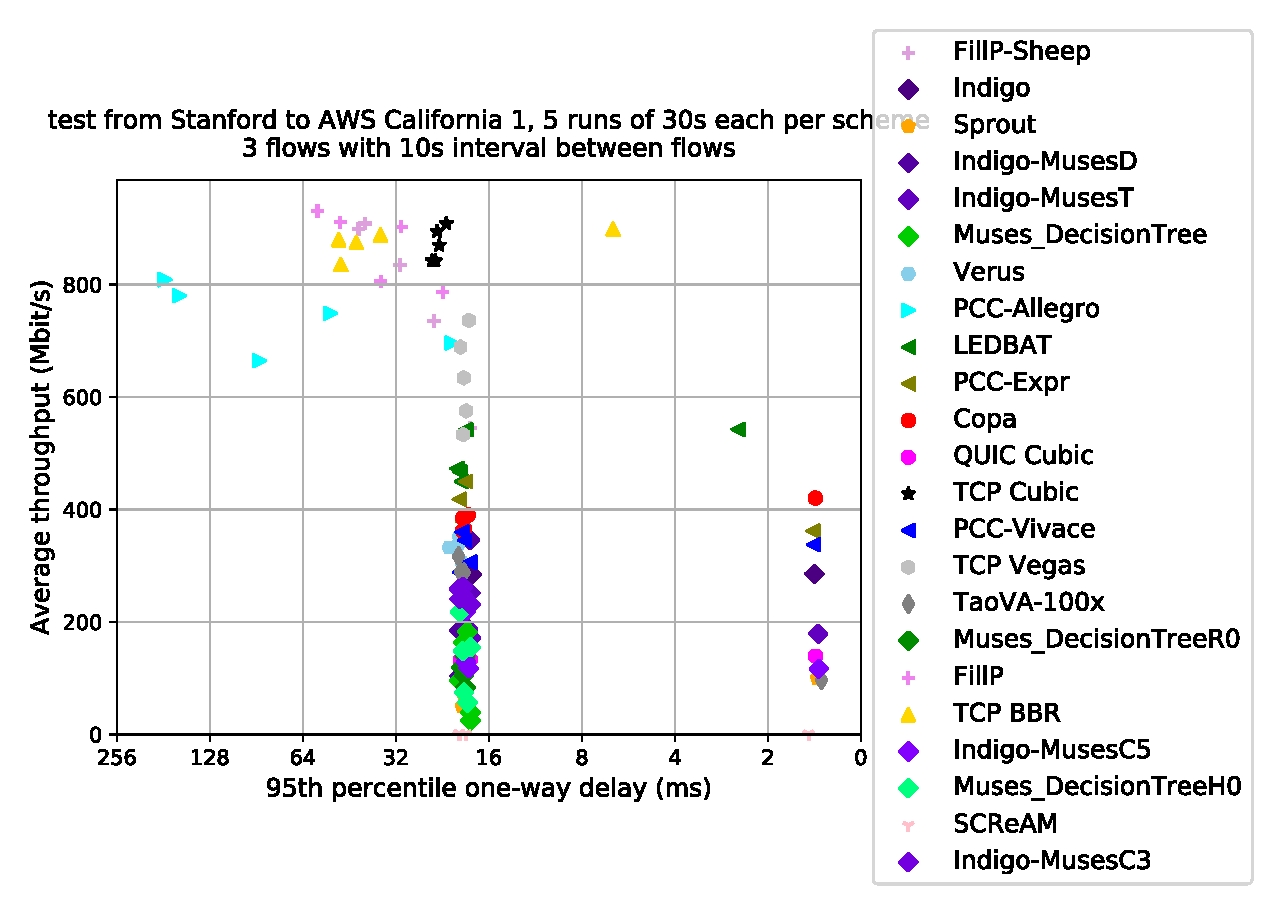
\includegraphics[width=\linewidth]{figures/chap02/measument-ccabr/cc.pdf}
  \caption{拥塞控制算法性能评测}
  \label{fig-measument-ccabr-cc}
\end{subfigure}%
\begin{subfigure}[t]{0.49\linewidth}
  \centering
  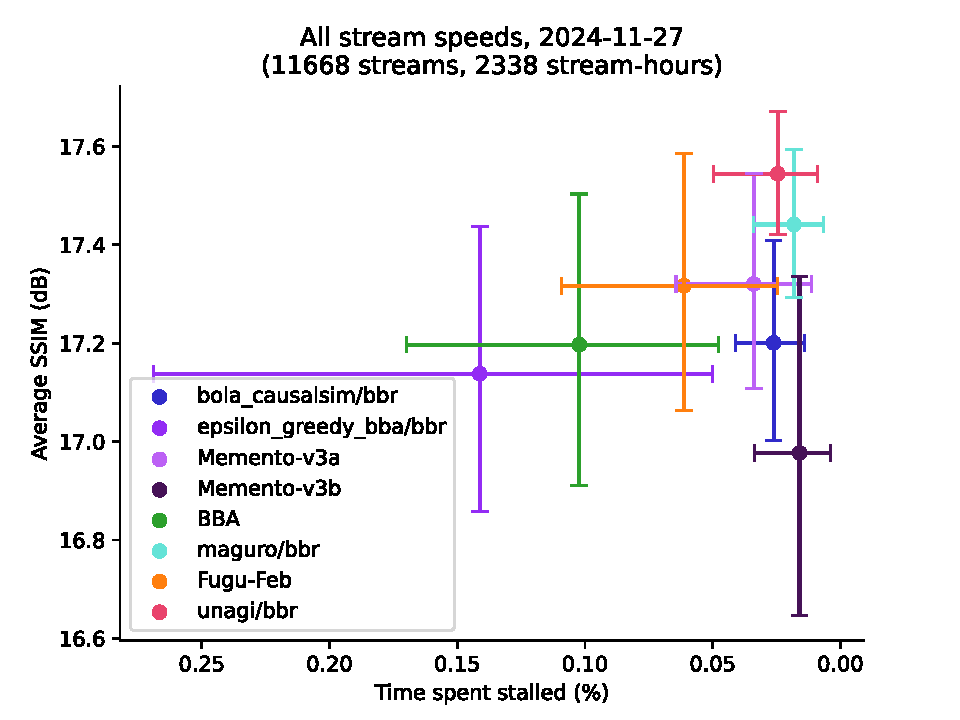
\includegraphics[width=\linewidth]{figures/chap02/measument-ccabr/abr.pdf}
  \caption{自适应码率算法性能评测}
  \label{fig-measument-ccabr-abr}
\end{subfigure}

\caption{Pantheon\cite{yan2018pantheon}和Puffer\cite{yan2020learning}的性能测量结果}
\label{fig-mea-ccabr}
\end{figure}


适配用户需求异质性和网络环境差异性的网络范式也在强化学习蓬勃发展后涌现。E2E \cite{zhang2019e2e}是第一个能够充分利用用户异质性来优化服务器资源分配的系统范式,包括各类发送速率控制算法和场景。E2E系统通过考虑不同用户对服务器端延迟的敏感性来调整资源分配,从而优化整体的QoE。Sage\cite{yen2023computers} 则将过去几十年来的所有拥塞算法的工作模式和行为通过强化学习的方式迁移到它自身身上,构建了拥有所有拥塞控制特性的一个强大的拥塞控制算法。

\section{强化学习领域框架概述}
\subsection{强化学习的基本概念和定义}
强化学习(Reinforcement learning,RL)是一种人工智能范式,涉及智能体(Agent)与环境(Environment)之间的交互,目的是最大化奖励函数 \cite{mnih2015human}。智能体与环境之间持续交互,在此框架下逐步学习,最终习得最优决策策略。

在强化学习中,所有环境中可能观察到的结果形成状态空间 $\mathcal{S}$,它描述了智能体在任一时间点可能观察到的环境状态信息。智能体维护一个策略 $\pi$,该策略定义了智能体在给定状态下采取不同动作的概率分布。智能体根据环境当前状态 $s_t$ 在每个离散时间步 $t$ 决定采取一个动作 $a_t$。所有可以执行的动作构成动作空间 $\mathcal{A}$。一旦环境接收到智能体的动作 $a_t$,它会生成一个奖励信号 $r_t$ 并转移到新的状态 $s_{t+1}$。这个过程不断重复,最终学习到一个策略 $\pi(\mathcal{A}|\mathcal{S})$,该策略最大化奖励的折现总和,这个折现总和用回报 $R_t$ 表示,如式\eqref{eq:rl-reward}所示:
\begin{equation}
\begin{aligned}
    R_t = \sum_{i=t}^{T}\gamma^{i-t}r(s_i,a_i) = r_t + \gamma r_{t+1} + ... + \gamma^{T-t}r_T,
\end{aligned}
\label{eq:rl-reward}
\end{equation}
其中,$\gamma$ 是折扣因子,用于确定短期奖励的优先级。折扣因子 $\gamma$ 的值通常在 $[0, 1]$ 范围内,越接近 1,表示智能体更重视长期回报;而接近 0 时,智能体则更关注近期的回报。在强化学习中,$\gamma$ 调整了未来奖励对当前决策的影响程度。通过合理选择 $\gamma$ 的值,可以平衡探索短期和长期回报之间的关系,帮助智能体制定合适的策略。

强化学习通过学习找到一个最优策略 $\pi_\phi$,其参数为 $\phi$,该策略最大化期望回报。具体来说,强化学习的目标是通过调整策略的参数 $\phi$,使得期望回报(即长期奖励的总和)达到最大。这个过程通常通过优化式\eqref{eq:rl-Jtheta}所示的目标函数来实现:
\begin{equation}
\begin{aligned}
    J(\phi) = \mathbb{E}_{s_i \sim p_\pi, a_i \sim \pi}[R_0].
\end{aligned}
\label{eq:rl-Jtheta}
\end{equation} 

\subsection{强化学习Actor-Critic架构}
在演员-评论家(Actor-Critic)架构中,包含两个网络:演员网络(Actor)和评论家网络(Critic)。演员网络学习最优的策略函数 $\pi_\phi(\mathcal{A}|\mathcal{S})$,旨在学习一个能够生成高奖励并与环境互动的策略。演员使用深度确定性策略梯度(Deep Deterministic Policy Gradient,DDPG)算法 \cite{silver2014deterministic} 来更新策略梯度。具体地,DDPG 是一种适用于连续动作空间的强化学习算法,通过策略梯度更新算法来改进策略,如式\eqref{eq:rl-nablaphi}所示:
\begin{equation}
\begin{aligned}
    \nabla_\phi J(\phi)=\mathbb{E}_{s\sim p_\pi}\left[\nabla_aQ^{\pi}(s,a)|_{a=\pi(s)}\nabla_\phi\pi_\phi(s)\right].
\end{aligned}
\label{eq:rl-nablaphi}
\end{equation} 

评论家网络(Critic network)估计当前策略的价值函数,评估演员(Actor)网络的性能。评论家网络通过式\eqref{eq:rl-qpitheta}表示:
\begin{equation}
\begin{aligned}
   Q^\pi(s,a)~=~\mathbb{E}_{s_i\sim p_\pi,a_i\sim\pi}\left[R_t|s,a\right].
\end{aligned}
\label{eq:rl-qpitheta}
\end{equation} 

为了限制在演员-评论家架构中的过度估计现象,提出了双延迟深度确定性策略梯度(Twin Delayed Deep Deterministic Policy Gradient, TD3)\cite{fujimoto2018addressing},以实现更高效的训练。



\subsection{强化学习Decision Transformer架构}
Decision Transformer\cite{chen2021decision}是由Lili Chen等人提出的一个强化学习范式,它的工作架构和状态、动作、奖励空间编码示意如图\ref{fig:decision_trans_archi}所示。

\begin{figure} [ht]
\centering
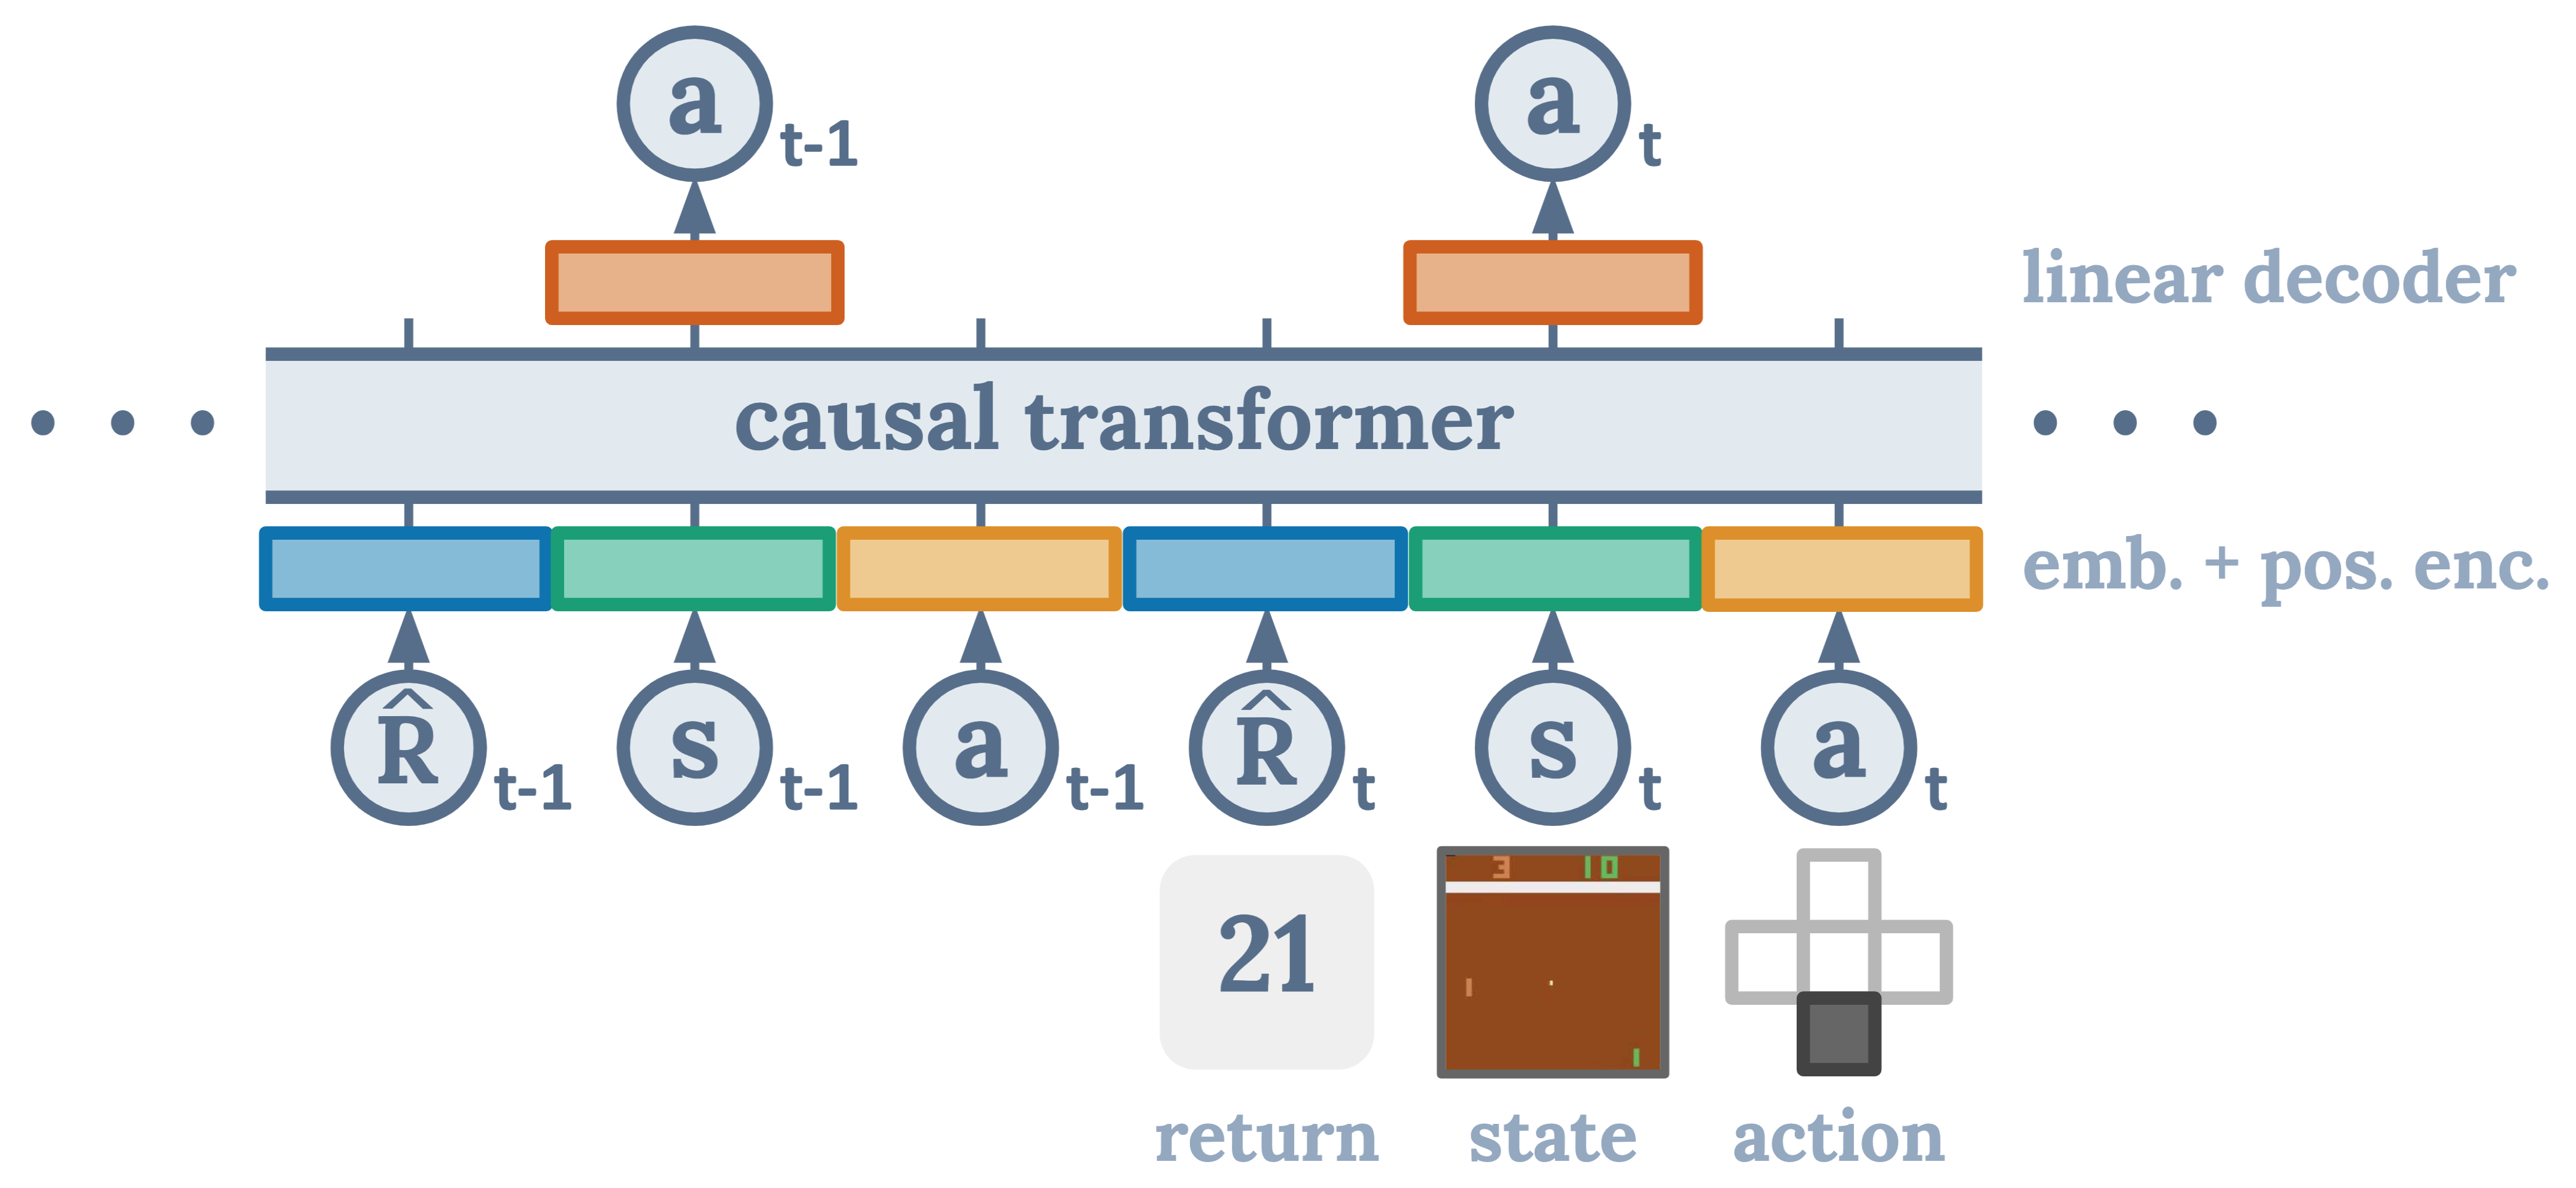
\includegraphics[width=0.8\textwidth]{figures/chap02/decision_transformer.png} 
\caption{Decision Transformer范式的工作框架\cite{chen2021decision}}
\label{fig:decision_trans_archi}
\end{figure}

Decision Transformer将一个将强化学习空间抽象为一个序列建模(Sequence Modeling)问题的框架,这有助于在模型选择时使用Transformer架构的模型,例如BERT\cite{koroteev2021bert}和GPT\cite{achiam2023gpt}类预训练大型语言模型,通过大规模并行的方式加快训练过程,并充分利用语言类生成模型的能力。

Decision Transformer相较于传统强化学习使用值函数(Q-Learning)或者策略梯度(Policy Gradient)的方式进行动作预测采用了截然不同的方式,它使用自回归的方式完成预测。通过将状态、动作和预期回报(Return-To-Go,RTG)编码成序列,Decision Transformer可以在不交互训练的情况下完成对最优动作的选择。



从图\ref{fig:decision_trans_archi}中可知,一个决策序列的预期回报(Return-To-Go,RTG)、状态(State)、动作(Action)按照时间先后通过特别的嵌入层(Embedding),并配置了对应的位置编码,通过一个Transformer类的模型通过一个线性映射层,输出了最新决策的动作。对应的状态转移、预期奖励和该动作又被作为下一个三元组继续进行动作决策,以自回归的方式做出新的决策。更具体的形式化描述可以表述为下列推导。

设定一个强化学习的序列状态 $s_t$、动作 $a_t$ 和奖励 $r_t$,其中$t$代表序列的决策时刻$1,2,...,T$,Decision Transformer利用该序列构建式\eqref{eq:three_deci}表示的三元组:
\begin{equation}
\begin{aligned}
    (R_1,s_1,a_1,R_2,s_2,a_2,...,R_T,s_T,a_T),
\end{aligned}
\label{eq:three_deci}
\end{equation} 

其中$R_t$代表Return-to-go,是Decision Transformer中特别的回报计算方式,统计从时间步$t$到终止时刻$T$的累计回报,用于告知模型优化的方向,如式\eqref{eq:rtg}所示:
\begin{equation}
\begin{aligned}
    R_t = r_t + \gamma r_{t+1} + \gamma^2 r_{t+2} + ... + \gamma ^{T-t}r_{T}.
\end{aligned}
\label{eq:rtg}
\end{equation} 

随后,$R_t$、动作 $a_t$ 和奖励 $r_t$分别通过各自的嵌入(Embedding)层完成到模型输入层的映射,并通过一个基于Transformer架构的模型,获得最终的输出动作决策。

Decision Transformer模型的预测是自回归的,给定过去的信息和目标回报,来预测当前的最优动作$\hat{a}_t$,可表示为式\eqref{eq:deci_at_goal}:
\begin{equation}
\begin{aligned}
    \hat{a}_t = f(R_t,s_t|R_{t-1},s_{t-1},a_{t-1},...).
\end{aligned}
\label{eq:deci_at_goal}
\end{equation} 


Decision Transformer训练时需要习得一个能够根据历史轨迹生成最优动作的策略,不通过实时与环境交互的方式,而是采用了有标签的监督学习方式进行训练,因此该方案更适配离线强化学习。其训练目标,即最小化的损失函数可以表示为式\eqref{eq:deci_trans_goal}:
\begin{equation}
\begin{aligned}
    L(\phi) = \mathbb{E}_{(R_t,s_t,a_t) \sim \mathcal{D}}\left[||a_t-\hat{a}_t||^2\right],
\end{aligned}
\label{eq:deci_trans_goal}
\end{equation}

其中$\mathcal{D}$是预先采集的离线强化学习决策轨迹构成的数据集,该数据集应该具有已经定义的奖励值作为选择评判标准;$a_t$ 表数据集中真实执行的动作,可能非最优解,亦作为部份轨迹使模型更全面习得决策结果的优缺点;$\hat{a}_t$则表示模型推测的结果。通过计算两个动作之间的L2范数平方误差,获得损失值,并最小化此损失值达成训练模型的目的。这种使用监督学习的方式能够避免贝尔曼方程计算的传播误差,直接建模了最优动作,同时利用了Transformer的长上下文感知特性,从而最大化了长期回报。

